\scanpage{25}
\uline{Lemme de Cartan}

$\unsure{\mathbb T|T}$ \deleted{\unsure{un}} site, \deleted{$S\in\unsure{\mathrm{Ob}\,T|T}$}

$F$ faisceau abélien sur $T$

$n\in\mathbb Z$

\deleted{$\mathcal U\inserted{\unsure{=(U_i^\alpha)}}$ famille \unsure{filtrante} croissante de rec. de $S$\inserted{\unsure{cofinale}},}

$\mathcal M$ sous-ens de $\operatorname{Ob}T$ \deleted{formé de}
\deleted{tt}
\inserted{\figure{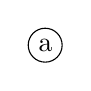
\begin{tikzpicture}[baseline=(n.base)]\node[draw,circle,inner sep=2pt] (n) {a};\end{tikzpicture}} $\mathcal M$ stable par produits finis}

On suppose \deleted{que}\inserted{\figure{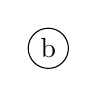
\begin{tikzpicture}[baseline=(n.base)]\node[draw,circle,inner sep=2pt] (n) {b};\end{tikzpicture}}}
pour tt $S\in\deleted{\unsure{\operatorname{Ob}T}}\inserted{\mathcal M}$, \deleted{\unsure{il existe}}
les \uline{recouvrements} de $S$ formés par des $\in\mathcal M$ sont
cofinaux pour les rec [il suffit \unsure{$=$}, qu'ils
suffisent à effacer \deleted{$\unsure{H^q(S,)}$} tt classe
de $H^q(\unsure{S|U},F)$, $0<q\leq n$.].

\margin{\figure{\begin{tikzpicture}[x=1cm,y=1cm]
\draw[thin] (.1,4.6) .. controls (1.2,4.4) and (2.2,4.35) .. (3.1,4.5);
\draw[line width=.6pt] (0,4.4) .. controls (-.08,3.5) and (.18,2.8) .. (.08,2.2);
\draw[thin] (.06,4.42) .. controls (.14,4.1) and (.1,3.9) .. (.03,3.6);
\draw[thin] (.1,2.15) .. controls (.18,1.2) and (.26,.4) .. (.26,0);
\draw[thin] (2.2,.5)--(4.3,2.6);
\node at (.18,2.75) {$\unsure{*}$};
\end{tikzpicture}}}

Conditions équivalentes

(i) $\forall S\in\mathcal M$, $H^i(S,F)=0$ pour $0<i\leq n$

(ii) $\forall S\in\mathcal M$, \deleted{\unsure{tout}} et tt rec.\inserted{$\mathcal U$} de $S$
formé par des $S_i\in\mathcal M$, on a
\[
\check H^i(\mathcal U,F)=0\quad\text{pour }0<i\leq n
\]

(iii) $\forall S\in\mathcal M$, on a
\[
\varinjlim_{\mathcal U}\check H^i(\mathcal U,F)=0\quad\text{pour }0<i\leq n
\]
où $\mathcal U$ varie sur les rec de $S$ formés
d'objets $\in\mathcal M$
\margin{\figure{\begin{tikzpicture}\draw (0,2.2)--(0,1.8);\draw (.04,.6)--(.07,0);\end{tikzpicture}}}
\margin{24}

